\chapter{Background}\label{ch:Background}

\section{Sparse Representation and Dictionary Learning}

Let $\mathbf{F} = [F_1$, $F_2$, $\dots F_d]$ be a set of $d$ features $F$ which are collected or curated. The goal is to rank the feature set $\mathbf{F}$ by evaluating a mean-removed training set of $n$ samples: $\mathbf{\bar{Y}} = [y_1$, $y_2$, $\dots, y_n] \in \mathbb{R}^{d \times n}$. The set of $k$ classes is defined as $\mathbf{C} = [C_1$, $C_2$, $\dots, C_k]$, where each of the $x$ samples is assigned to a class $C$. In sparse representation the input sample is represented as a linear combination of dictionary elements $D$ in a over-complete ($d \ll m$) dictionary $\mathbf{D} = [D_1, D_2, \dots, D_m] \in \mathbb{R}^{d \times m}$, where the number of dictionary elements used, $s$, is far less than the number of dictionary atoms: $s \ll m$. The set coefficients $\bm{\alpha} = [\alpha_1, \alpha_2, \dots, \alpha_n] \in \mathbb{R}^{m \times n}$ of the linear combination is called the sparse coefficients. Each coefficient vector contains $s$ nonzero entries; the remaining $m-s$ entries are exactly zero. The general objective function used for calculating the sparse representation is given by (\ref{eq:sparse}) with an $\ell_0$ constraint on sparsity.

\begin{equation}
    \label{eq:sparse}
    \argmin_{\mathbf{D},\bm{\alpha}} ||\mathbf{\bar{X}}- \mathbf{D}\bm{\alpha}||_F + ||\bm{\alpha}||_0
\end{equation}

The KSVD algorithm is an efficient iterative method that solves the objective function by, first fixing the $\mathbf{D}$ and optimizing the $\bm{\alpha}$ using orthogonal matching pursuit (OMP)\cite{Pati1993}. Second, it fixes $\bm{\alpha}$ then optimize $\mathbf{D}$ with generalized K-means and singular value decomposition (SVD). Figure\ref{fig: DictLearn} represent the input signal, learned dictionary, and the sparse coding as a matrix. Since the learned dictionary is over-complete, the spread of the dictionary atoms can give an insight into which features are more relevant for the representation. Hence, we will be defining simple metrics that will quantify the spread of the dictionary elements in each of the features. 

% \begin{figure}
%     \centering
%     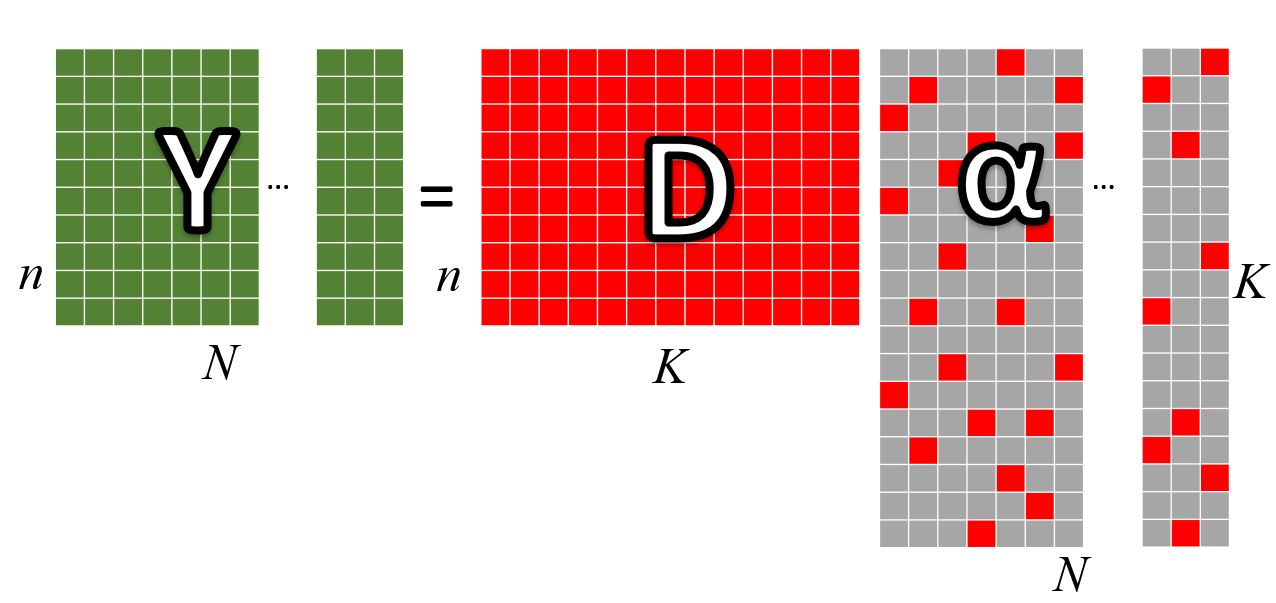
\includegraphics[width = 0.4\textwidth]{figures/DictLearn.JPG}
%     \caption{Matrix representation of the input signal, learned dictionary, and the sparse coefficients}\label{fig: DictLearn}
% \end{figure}

In LC-KSVD\cite{Jiang2011}, the algorithm employs an objective function comprised of reconstructive, discriminative, and classification costs. The LC-KSVD dictionary is initiated by equally dividing among the classes. Then class labels are used to force the dictionary atom learning to be constrained into the predefined dictionary locations. However, this method does not takes into account class imbalances.

Frozen dictionary learning is a modification of traditional sparse coding dictionary learning that attempts to learn a dictionary that can effectively model imbalanced datasets\cite{Carroll2017}. In this algorithm first, the dictionary learning step is carried out using an algorithm, then the learned dictionary elements are held constant and the dictionary is augmented with additional elements. For the next step, the dictionary is trained again on data containing abnormalities. The frozen elements of the dictionary represent the normal aspects of the data, hence the new elements (non-frozen) learn to represent the anomalous aspects of the data that are not present in the normal data. The frozen dictionary approach could be generally used and applied to the problems including data with or without abnormalities. 

% \begin{figure}
% \begin{centering}
%     \subfloat[][]{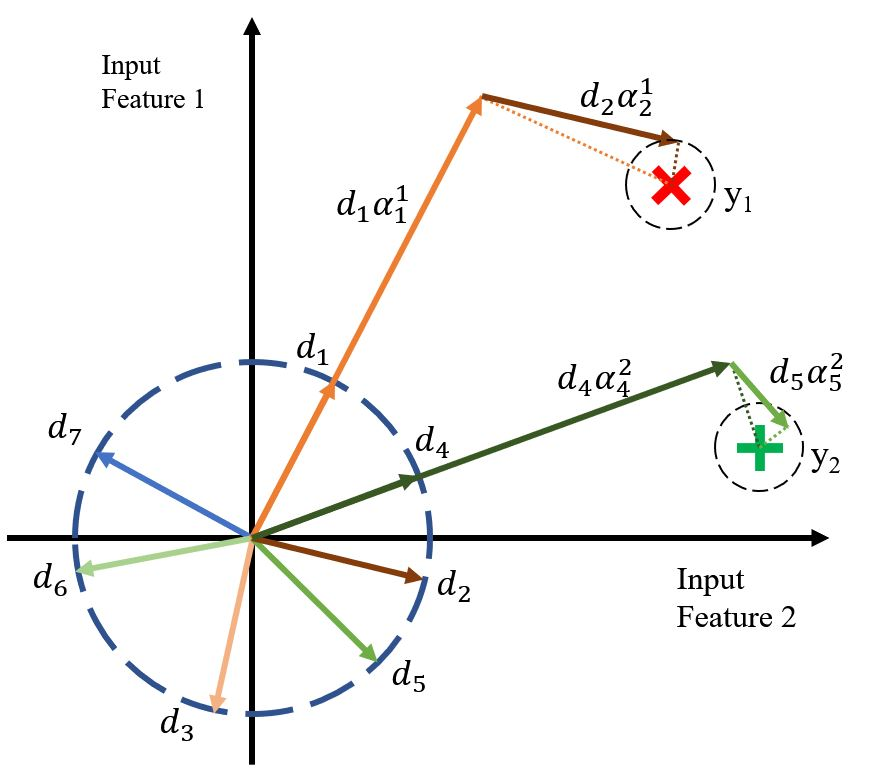
\includegraphics[width=.4\textwidth]{Input domain.JPG}\label{fig:Indomain}}
%     \qquad
%     \subfloat[][]{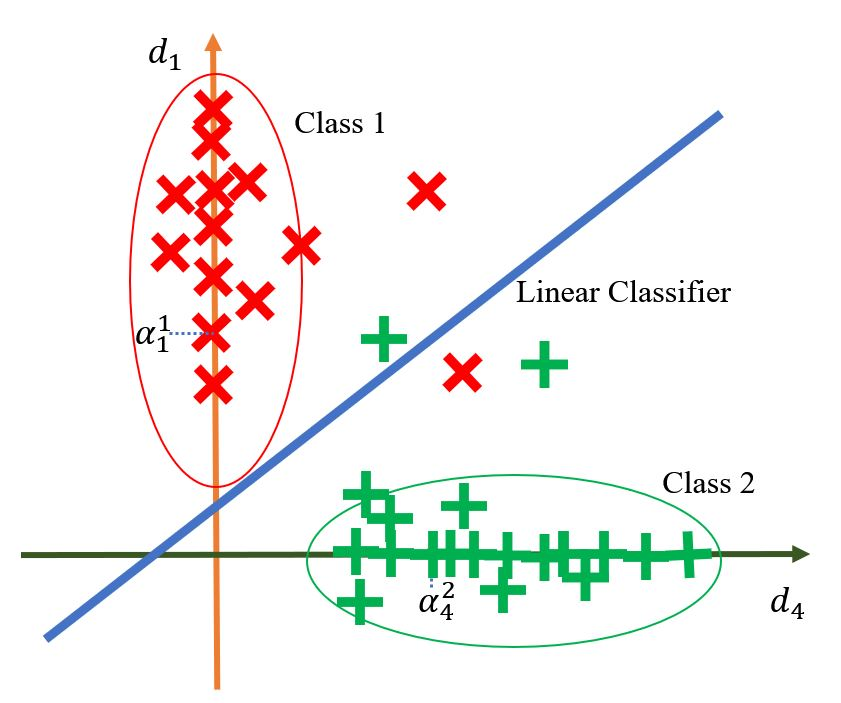
\includegraphics[width=.4\textwidth]{Dict domain.JPG}\label{fig:Dictdomain}}
%     % \subsection{Dictionary atoms domain}
    
%     \caption{(a) Sparse representation of the input data with dictionary atoms. (b) Classifier in the dictionary atoms domain.}\label{fig:image2}
% \end{centering}
% \end{figure}


Figure\ref{fig:Indomain} illustrates the representation of the input signals with the learned dictionary atoms in a two-dimensional input feature domain with sparsity, $S =2$. $y_1$, $y_2$ are the input signals belonging to two separate classes. With LC-KSVD the algorithm forces dictionary atoms $d_1, \dots , d_3$ to be used for $y_1$ in class 1 and $d_4, \dots , d_6$ to be used for $y_2$ in class 2. Fig.\ref{fig:Dictdomain} illustrates the learned classifier boundary in the (sparse) domain of $d_1$ and $d_4$. Due to the class constraints in the dictionary learning process, the majority of the input data will only be represented by the dictionary atoms corresponding to their class. Thus in the sparse domain, most signals will lie in a class-specific subspace of the entire dictionary. Hence, a linear classifier can be utilized for the classification with satisfactory results. Further, there is a direct relationship between the classifier domain and the input domain. 